% !TeX program = pdflatex
% =============================================================================
% Arbeitsblatt: Magnetfelder
% UZH Praktikum I -- Sara Romer Urban, Kantonsschule im Lee, HS2026
% Klasse: 4fh (01.09.2026, nur 4fh -- 4cdeg hat hier Hospitation, kein
% eigenes Dokument noetig).
%
% Ablauf (direkt mit Loris per Chat abgestimmt, 31.08.2026 -- ersetzt die
% Reihenfolge aus einer frueheren Fassung dieser Datei):
%   0. Kurze Definition "Magnetfeld" (Stand 03.09.2026, neu).
%   1. Repetition Magnete/Kompassnadel: Zeichenuebung "Kompassnadeln
%      einzeichnen" (sechs Kreise, TikZ-Skizze zweier zugewandter
%      Stabmagnete); das Foto zwei_magnete.png dient nur noch als
%      zusaetzliche Loesung zum Vergleich (Stand 03.09.2026 ueberarbeitet
%      -- die fruehere separate Bildfrage-Aufgabe wurde entfernt).
%   2. Vergleich elektrisches Punktladungsfeld vs. Stabmagnetfeld.
%   3. Regeln zum Zeichnen von Feldlinien + Zeichenuebung (zwei Stabmagnete,
%      gleichnamige Pole zueinander).
%   4. Erdmagnetfeld.
%   5. Oersted-Geschichte (kurz, als Ueberleitung).
%   6. Baukasten-Experiment (Partnerarbeit): Stromkreis mit Stableiter und
%      Spule, Feld mit kleinen Kompassnadeln erkunden, danach Stromrichtung
%      umkehren -- bewusst VOR der Theorie (entdeckendes Lernen).
%   7. Theorie: Rechte-Faust-Regel + Formeln fuer geraden Leiter und Spule.
%   8. Ein paar Aufgaben (Formelanwendung).
%
% Ring/Helmholtz-Spule, Ringspule (Toroid) und die Permeabilitaets-
% Sortieraufgabe sind auf Loris' ausdruecklichen Wunsch NICHT mehr Teil
% dieser Doppellektion (Stand 31.08.2026) -- lernziele.md (LZ3/LZ4) und
% magnetfelder-lektionsplan.tex sind entsprechend VERALTET und muessen noch
% separat nachgezogen werden, bevor sie wieder als Quelle fuer dieses
% Dokument gelten.
%
% Stand 03.09.2026: Bilder fuer alle Abschnitte liegen inzwischen vor
% (zwei_magnete.png, elektrisches_fled_punktladungen.jpg,
% magnetfeld_permanentmagnet.png, erdmagnetfeld.png,
% Erdmagnetfeld-innen-scaled.jpg bei der Spule als Analogie, leiter.png,
% spule.png). Die Formeln fuer B (gerader Leiter, Spule) stehen auf
% Wunsch direkt im Fliesstext -- keine Fill-in-the-blank-Antwortbox mehr,
% die SuS sollen sie nicht mehr selbst herleiten.
%
% Quellen: Vorwissen/Magnetismus/Werkstatt_Magnetismus.docx
% (15-Posten-Werkstatt, bereits bekannt), PhysikLibre Kap. 13.1/13.4 (dieser
% Ordner), LEIFIphysik (Magnetfeld gerader Leiter/Zylinderspule).
% =============================================================================
\documentclass[addpoints,11pt,a4paper]{exam}

\usepackage[T1]{fontenc}
\usepackage[utf8]{inputenc}
\usepackage[ngerman]{babel}
\usepackage{lmodern}
\usepackage[a4paper,margin=2.2cm,headheight=14pt]{geometry}
\usepackage{amsmath}
\usepackage{amssymb}
\usepackage{siunitx}
% Hausstil: zusammengesetzte Einheiten immer als echter Bruch (\frac), nicht
% als Inline-Schrägstrich oder \tfrac -- gilt global für jedes \si/\SI.
\sisetup{per-mode=fraction,fraction-command=\frac}
\usepackage{array,booktabs,tabularx,multirow}
\usepackage{enumitem}
\usepackage{xcolor}
\usepackage{colortbl}
\usepackage{tikz}
\usepackage{physics}
\usepackage{circuitikz}
\usepackage[most]{tcolorbox}
\usepackage{lastpage}
\usepackage{graphicx}
\usepackage{hyperref}

\usetikzlibrary{arrows.meta,calc,angles,quotes,decorations.markings}

\usepackage{setspace}
\usepackage{needspace}
\setlength{\parindent}{0pt}
\setlength{\parskip}{0.6em}
\setstretch{1.08}
\setlist[itemize]{itemsep=0.4em}

% -----------------------------
% Farben (Corporate-Farbschema Physik KFR)
% -----------------------------
\definecolor{titleblue}{HTML}{183A6B}
\definecolor{accentblue}{HTML}{2E6F9E}
\definecolor{lightblue}{HTML}{EAF4FB}
\definecolor{verylightblue}{HTML}{F7FBFE}
\definecolor{lightgray}{HTML}{F4F6F8}
\definecolor{darkgray}{HTML}{4A4A4A}
\definecolor{accentorange}{HTML}{D9720C}
\definecolor{accentpurple}{HTML}{7B2D8E}
% Theorie-Block: eigene Farbe (grün).
\definecolor{theorygreen}{HTML}{2E7D4F}
\definecolor{lighttheorygreen}{HTML}{EAF7EF}
% Gruppenarbeit-Box: eigene Farbe (Petrol/Teal).
\definecolor{groupteal}{HTML}{1B7F72}
\definecolor{lightgroupteal}{HTML}{E8F5F3}
% Hinweisbox: Orange (accentorange), für wichtige Klarstellungen.
\definecolor{lightorange}{HTML}{FCEEE0}
% Formelbox: Violett (accentpurple), für die zentralen Formeln dieser Einheit.
\definecolor{lightpurple}{HTML}{F3EAF7}

% Links (hyperref): farblich ans Corporate-Farbschema angeglichen.
\hypersetup{
  colorlinks=true,
  urlcolor=accentblue,
  linkcolor=accentblue,
  pdftitle={Arbeitsblatt 5: Magnetfelder},
  pdfauthor={Loris Keller}
}

% -----------------------------
% Spaltentypen
% -----------------------------
\newcolumntype{Y}{>{\centering\arraybackslash}X}
\newcolumntype{P}[1]{>{\raggedright\arraybackslash}p{#1}}

% -----------------------------
% Boxen
% -----------------------------
\tcbset{before skip=10pt, after skip=10pt}
\newtcolorbox{titlebox}{
  enhanced,
  colback=titleblue,
  colframe=titleblue,
  boxrule=0pt,
  arc=3mm,
  left=3mm,right=3mm,top=3mm,bottom=3mm
}

\newlength{\aufgabenindent}
\settowidth{\aufgabenindent}{10.\hskip\labelsep}

% Praktikum I: Lernziele/Einleitung/Theorie/Aufgaben werden NICHT mehr
% farbig gerahmt (nur Formel-, Hinweis- und Antwortbox bleiben Boxen) --
% siehe institutionen/UZH-Praktikum-I/CLAUDE.md, Abschnitt "Boxen-Layout".
\newenvironment{infobox}{%
  \par\addvspace{10pt}\noindent
}{%
  \par\addvspace{10pt}
}

\newenvironment{theoriebox}[1][Theorie]{%
  \par\addvspace{10pt}\noindent\textbf{#1}\par\smallskip\noindent
}{%
  \par\addvspace{10pt}
}

% taskbox/groupbox stehen in questions VOR dem ersten \question (Bilder,
% Fliesstext) -- exam.cls' questions-Liste braucht dafür eine echte,
% eigenständige Box (sonst "Something's wrong--perhaps a missing \item",
% weil z.B. ein \begin{center} vor dem ersten \item der Aussenliste steht).
% Deshalb bleiben es tcolorboxen, nur unsichtbar gemacht (keine Farbe/Rahmen,
% kein Padding) statt sie durch reine Absätze zu ersetzen.
\newtcolorbox{taskbox}[1][]{
  enhanced, breakable,
  colback=white, colframe=white, boxrule=0pt,
  left=0mm,right=0mm,top=0mm,bottom=0mm,
  before skip=10pt, after skip=10pt,
  before upper={%
    \def\tmpboxtitle{#1}%
    \ifx\tmpboxtitle\empty\else\noindent\textbf{#1}\par\smallskip\fi
  }
}

\newtcolorbox{groupbox}[1][Gruppenarbeit]{
  enhanced, breakable,
  colback=white, colframe=white, boxrule=0pt,
  left=0mm,right=0mm,top=0mm,bottom=0mm,
  before skip=10pt, after skip=10pt,
  before upper={\noindent\textbf{#1}\par\smallskip}
}

% beispielbox: für die Einleitung und für durchgerechnete Beispiele
% innerhalb der Theorie -- wie die anderen Inhaltsboxen ungerahmt.
\newenvironment{beispielbox}[1][Beispiel]{%
  \par\addvspace{10pt}\noindent\textbf{#1}\par\smallskip\noindent
}{%
  \par\addvspace{10pt}
}

% hinweisbox: Orange, für wichtige Klarstellungen/Verwechslungswarnungen.
\newtcolorbox{hinweisbox}[1][Hinweis]{
  enhanced,
  breakable,
  colback=lightorange,
  colframe=accentorange,
  title={#1},
  fonttitle=\bfseries,
  boxrule=0.7pt,
  arc=2mm,
  left=5mm,right=5mm,top=2mm,bottom=2mm
}

% formelbox: Violett, um die zentralen Formeln dieser Einheit hervorzuheben.
\newtcolorbox{formelbox}[1][Formel]{
  enhanced,
  breakable,
  colback=lightpurple,
  colframe=accentpurple,
  title={#1},
  fonttitle=\bfseries,
  boxrule=0.9pt,
  arc=2mm,
  left=5mm,right=5mm,top=2mm,bottom=2mm
}

\newtcolorbox{answerbox}{
  breakable,
  colback=white,
  colframe=gray!55,
  boxrule=0.5pt,
  arc=1.5mm,
  left=2mm,right=2mm,top=2mm,bottom=2mm
}

% teilkopf: fette Zwischenüberschrift zur klaren Abgrenzung der Teile
% innerhalb der langen Lernaufgabe -- ungerahmt, wie die anderen
% Inhaltsboxen.
\newenvironment{teilkopf}{%
  \par\addvspace{8pt}\noindent\bfseries\sffamily
}{%
  \par\addvspace{6pt}
}

% Marke: kleines farbiges Inline-Label für Teilschritte (z.B. "Schritt 1")
% und Ergebnis-Callouts innerhalb einer Aufgabe. Standardfarbe Violett (wie
% formelbox); über das optionale Argument umschaltbar, z.B. \Marke[accentorange]{...}.
\newtcbox{\Marke}[1][accentpurple]{
  nobeforeafter,
  colback=#1,
  colframe=#1,
  coltext=white,
  boxrule=0pt,
  arc=2pt,
  left=5pt,right=5pt,top=2pt,bottom=2pt,
  fontupper=\bfseries\sffamily\small
}

% Kompasskreis/Kompassnadel: leerer Kreis (Aufgabe) bzw. Kreis mit Nadel in
% Richtung #3 (Lösung, Winkel in Grad, 0 = nach rechts) für die
% Kompassnadel-Zeichenübung bei Magnetfeldern.
\newcommand{\Kompasskreis}[2]{\draw[thick] (#1,#2) circle (0.38);}
\newcommand{\Kompassnadel}[3]{%
  \draw[thick] (#1,#2) circle (0.38);
  \draw[thick,-{Latex[length=2.2mm]}] ($(#1,#2)+(#3+180:0.28)$) -- ($(#1,#2)+(#3:0.28)$);
  \node[font=\scriptsize\bfseries] at ($(#1,#2)+(#3:0.58)$) {N};
}

% --- Lösungen ein-/ausblenden -----------------------------------------------
\noprintanswers
%\printanswers

\pointformat{}
\renewcommand{\solutiontitle}{\noindent\color{titleblue}\textbf{Lösung:}\enspace}

\pagestyle{headandfoot}
\cfoot{\textcolor{darkgray}{Seite \thepage\ von \pageref{LastPage}}}

\newcommand{\Kopfzeile}[4]{%
  \begin{titlebox}
    {\color{white}\sffamily\bfseries\Large #4}
  \end{titlebox}
  \vspace{0.5em}
  \noindent\textbf{Klasse:}~#1 \hfill \textbf{Datum:}~#2 \hfill \textbf{Thema:}~#3
    \hfill \textbf{Lehrperson:}~Loris Keller
  \vspace{0.8em}
  \lhead{\textcolor{darkgray}{#3}}
  \rhead{\textcolor{darkgray}{#4}}
}

\newlength{\antwortraumlen}
\newcommand{\Antwortraum}[1]{%
  \pgfmathsetlength{\antwortraumlen}{#1*2.5cm}%
  \begin{answerbox}
    \rule{0pt}{\antwortraumlen}%
  \end{answerbox}%
}

% Werte für Kopfzeile zentral setzen
\newcommand{\Klasse}{4fh}
\newcommand{\Datum}{01.09.2026}
\newcommand{\Thema}{Magnetfelder}
\newcommand{\ArbeitsblattTitel}{Arbeitsblatt 5: Magnetfelder}

\begin{document}

\Kopfzeile{\Klasse}{\Datum}{\Thema}{\ArbeitsblattTitel}

% =============================================================================
% Definition: Magnetfeld
% =============================================================================
\begin{theoriebox}[Magnetfeld: Definition]
\textbf{\emph{Ein Magnetfeld}} ist ein Modell für den Raum, in dem
magnetische Wirkungen auftreten.
\end{theoriebox}

% =============================================================================
% Kompassnadeln einzeichnen (Repetition; Foto als zusätzliche Lösung)
% =============================================================================
\begin{questions}
\begin{taskbox}[Kompassnadeln einzeichnen]
\question Zwei gleich starke Stabmagnete liegen sich gegenüber, dabei
sind ihr Nordpol (links) und ihr Südpol (rechts) einander zugewandt.
Zeichnen Sie in jeden der acht Kreise ein, wie sich eine dort platzierte
Kompassnadel ausrichten würde (Pfeil vom Süd- zum Nordpol der Nadel,
\glqq N\grqq{} am Nordpolende der Nadel).
\begin{answerbox}
\begin{center}
\begin{tikzpicture}[>=Latex,scale=1]
  % linker Magnet: S (links) -- N (rechts, zeigt zur Mitte)
  \draw[thick] (-4.5,0) rectangle (-2,0.9);
  \draw[thick] (-3.25,0) -- (-3.25,0.9);
  \node at (-3.875,0.45) {S};
  \node at (-2.625,0.45) {N};
  % rechter Magnet: S (links, zeigt zur Mitte) -- N (rechts)
  \draw[thick] (2,0) rectangle (4.5,0.9);
  \draw[thick] (3.25,0) -- (3.25,0.9);
  \node at (2.625,0.45) {S};
  \node at (3.875,0.45) {N};
  \Kompasskreis{0}{0.45}
  \Kompasskreis{-1.3}{1.9}
  \Kompasskreis{1.3}{1.9}
  \Kompasskreis{0}{-1.5}
  \Kompasskreis{-1.3}{-1.9}
  \Kompasskreis{1.3}{-1.9}
  \Kompasskreis{-5.3}{0.45}
  \Kompasskreis{5.3}{0.45}
\end{tikzpicture}
\end{center}
\end{answerbox}
\begin{solution}
\begin{center}
\begin{tikzpicture}[>=Latex,scale=1]
  \draw[thick] (-4.5,0) rectangle (-2,0.9);
  \draw[thick] (-3.25,0) -- (-3.25,0.9);
  \node at (-3.875,0.45) {S};
  \node at (-2.625,0.45) {N};
  \draw[thick] (2,0) rectangle (4.5,0.9);
  \draw[thick] (3.25,0) -- (3.25,0.9);
  \node at (2.625,0.45) {S};
  \node at (3.875,0.45) {N};
  \Kompassnadel{0}{0.45}{0}
  \Kompassnadel{-1.3}{1.9}{55}
  \Kompassnadel{1.3}{1.9}{-55}
  \Kompassnadel{0}{-1.5}{0}
  \Kompassnadel{-1.3}{-1.9}{-55}
  \Kompassnadel{1.3}{-1.9}{55}
  \Kompassnadel{-5.3}{0.45}{0}
  \Kompassnadel{5.3}{0.45}{0}
  \node at (0.55,1.05) {\scriptsize 1};
  \node at (-1.85,2.5) {\scriptsize 2};
  \node at (1.85,2.5) {\scriptsize 3};
  \node at (0.55,-1.95) {\scriptsize 4};
  \node at (-1.85,-2.5) {\scriptsize 5};
  \node at (1.85,-2.5) {\scriptsize 6};
  \node at (-4.75,1.05) {\scriptsize 7};
  \node at (5.85,1.05) {\scriptsize 8};
\end{tikzpicture}
\end{center}
Kreis 1 liegt genau auf der Linie zwischen den beiden zugewandten Polen.
Die Nadel zeigt dort waagrecht von Nord- zu Südpol. Kreis 2 liegt näher
am Nordpol und oberhalb der Mittellinie: Die Feldlinien treten dort
schräg nach oben aus dem Nordpol aus, bevor sie sich später Richtung
Südpol krümmen. Die Nadel zeigt entsprechend schräg nach oben rechts.
Kreis 3 liegt spiegelbildlich näher am Südpol: Dort krümmen sich die
Feldlinien bereits nach unten in den Südpol hinein, die Nadel zeigt
deshalb schräg nach unten rechts. Kreis 4 liegt unterhalb der Magnete auf
der Mittellinie. Dort verläuft das Feld wie bei Kreis 1 im Wesentlichen
waagrecht von Nord- zu Südpol. Die Kreise 5 und 6 liegen unterhalb der
Magnete, spiegelbildlich zu den Kreisen 2 und 3. Die Nadeln zeigen dort
ebenfalls schräg, allerdings mit vertauschter Neigung (Kreis 5 schräg
nach unten rechts, Kreis 6 schräg nach oben rechts). Die Kreise 7 und 8
liegen an den äusseren Enden der beiden Magnete, ausserhalb von ihnen,
aber ebenfalls auf der gemeinsamen Mittellinie -- dort zeigt die Nadel
wieder waagrecht nach rechts, genau wie bei Kreis 1: Auf der Achse eines
Magnetpaars zeigt das Feld sowohl zwischen als auch ausserhalb der Pole
stets in dieselbe Richtung.

Zum Vergleich: dieselbe Anordnung als Foto, mit einer echten Kompassnadel
auf der Mittellinie (entspricht Kreis 1).
\begin{center}
  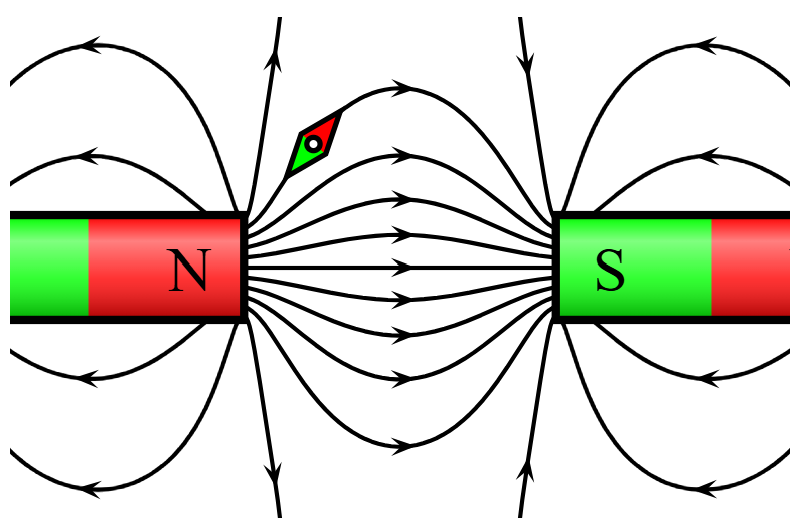
\includegraphics[width=7cm]{Bilder/zwei_magnete.png}
\end{center}
{\scriptsize Kompassnadel im Feld zwischen den einander zugewandten Polen
zweier Stabmagnete.}
\end{solution}
\end{taskbox}
\end{questions}

% =============================================================================
% Vergleich: elektrisches Punktladungsfeld vs. Stabmagnetfeld
% =============================================================================
\begin{questions}
\begin{taskbox}[Vergleich: Punktladungsfeld und Stabmagnetfeld]
\question Betrachten Sie die beiden Felder nebeneinander: links das
elektrische Feld zweier entgegengesetzter Punktladungen (ein elektrischer
Dipol, bereits aus der Elektrostatik bekannt), rechts das Magnetfeld eines
Stabmagneten (ebenfalls ein Dipol).
\begin{center}
% Höhe statt Breite angeglichen: Die beiden Bilder haben sehr
% unterschiedliche Seitenverhältnisse (Punktladungsfeld breit/flach,
% Stabmagnetfeld nahezu quadratisch) -- bei gleicher Breite wirkt das
% Stabmagnetfeld dadurch fast doppelt so gross wie das Punktladungsfeld.
% Gleiche Höhe ergibt einen tatsächlich vergleichbaren visuellen Eindruck.
\begin{minipage}[t]{9.6cm}\centering
  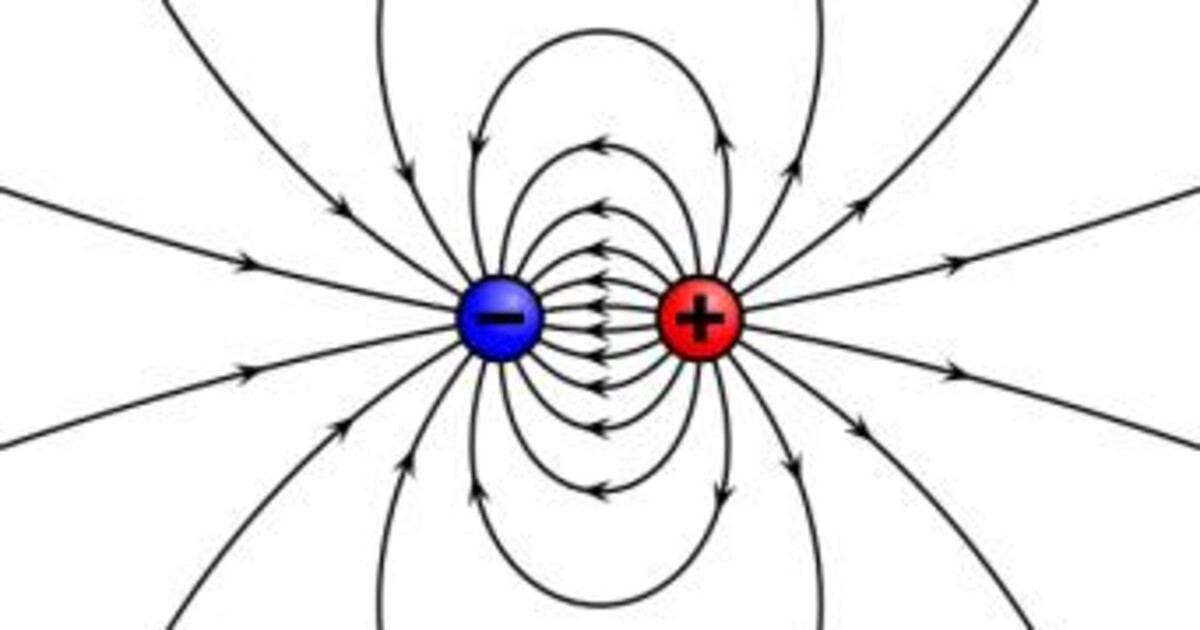
\includegraphics[height=5cm]{Bilder/elektrisches_fled_punktladungen.jpg}\\
  elektrischer Dipol
\end{minipage}\hfill
\begin{minipage}[t]{6.2cm}\centering
  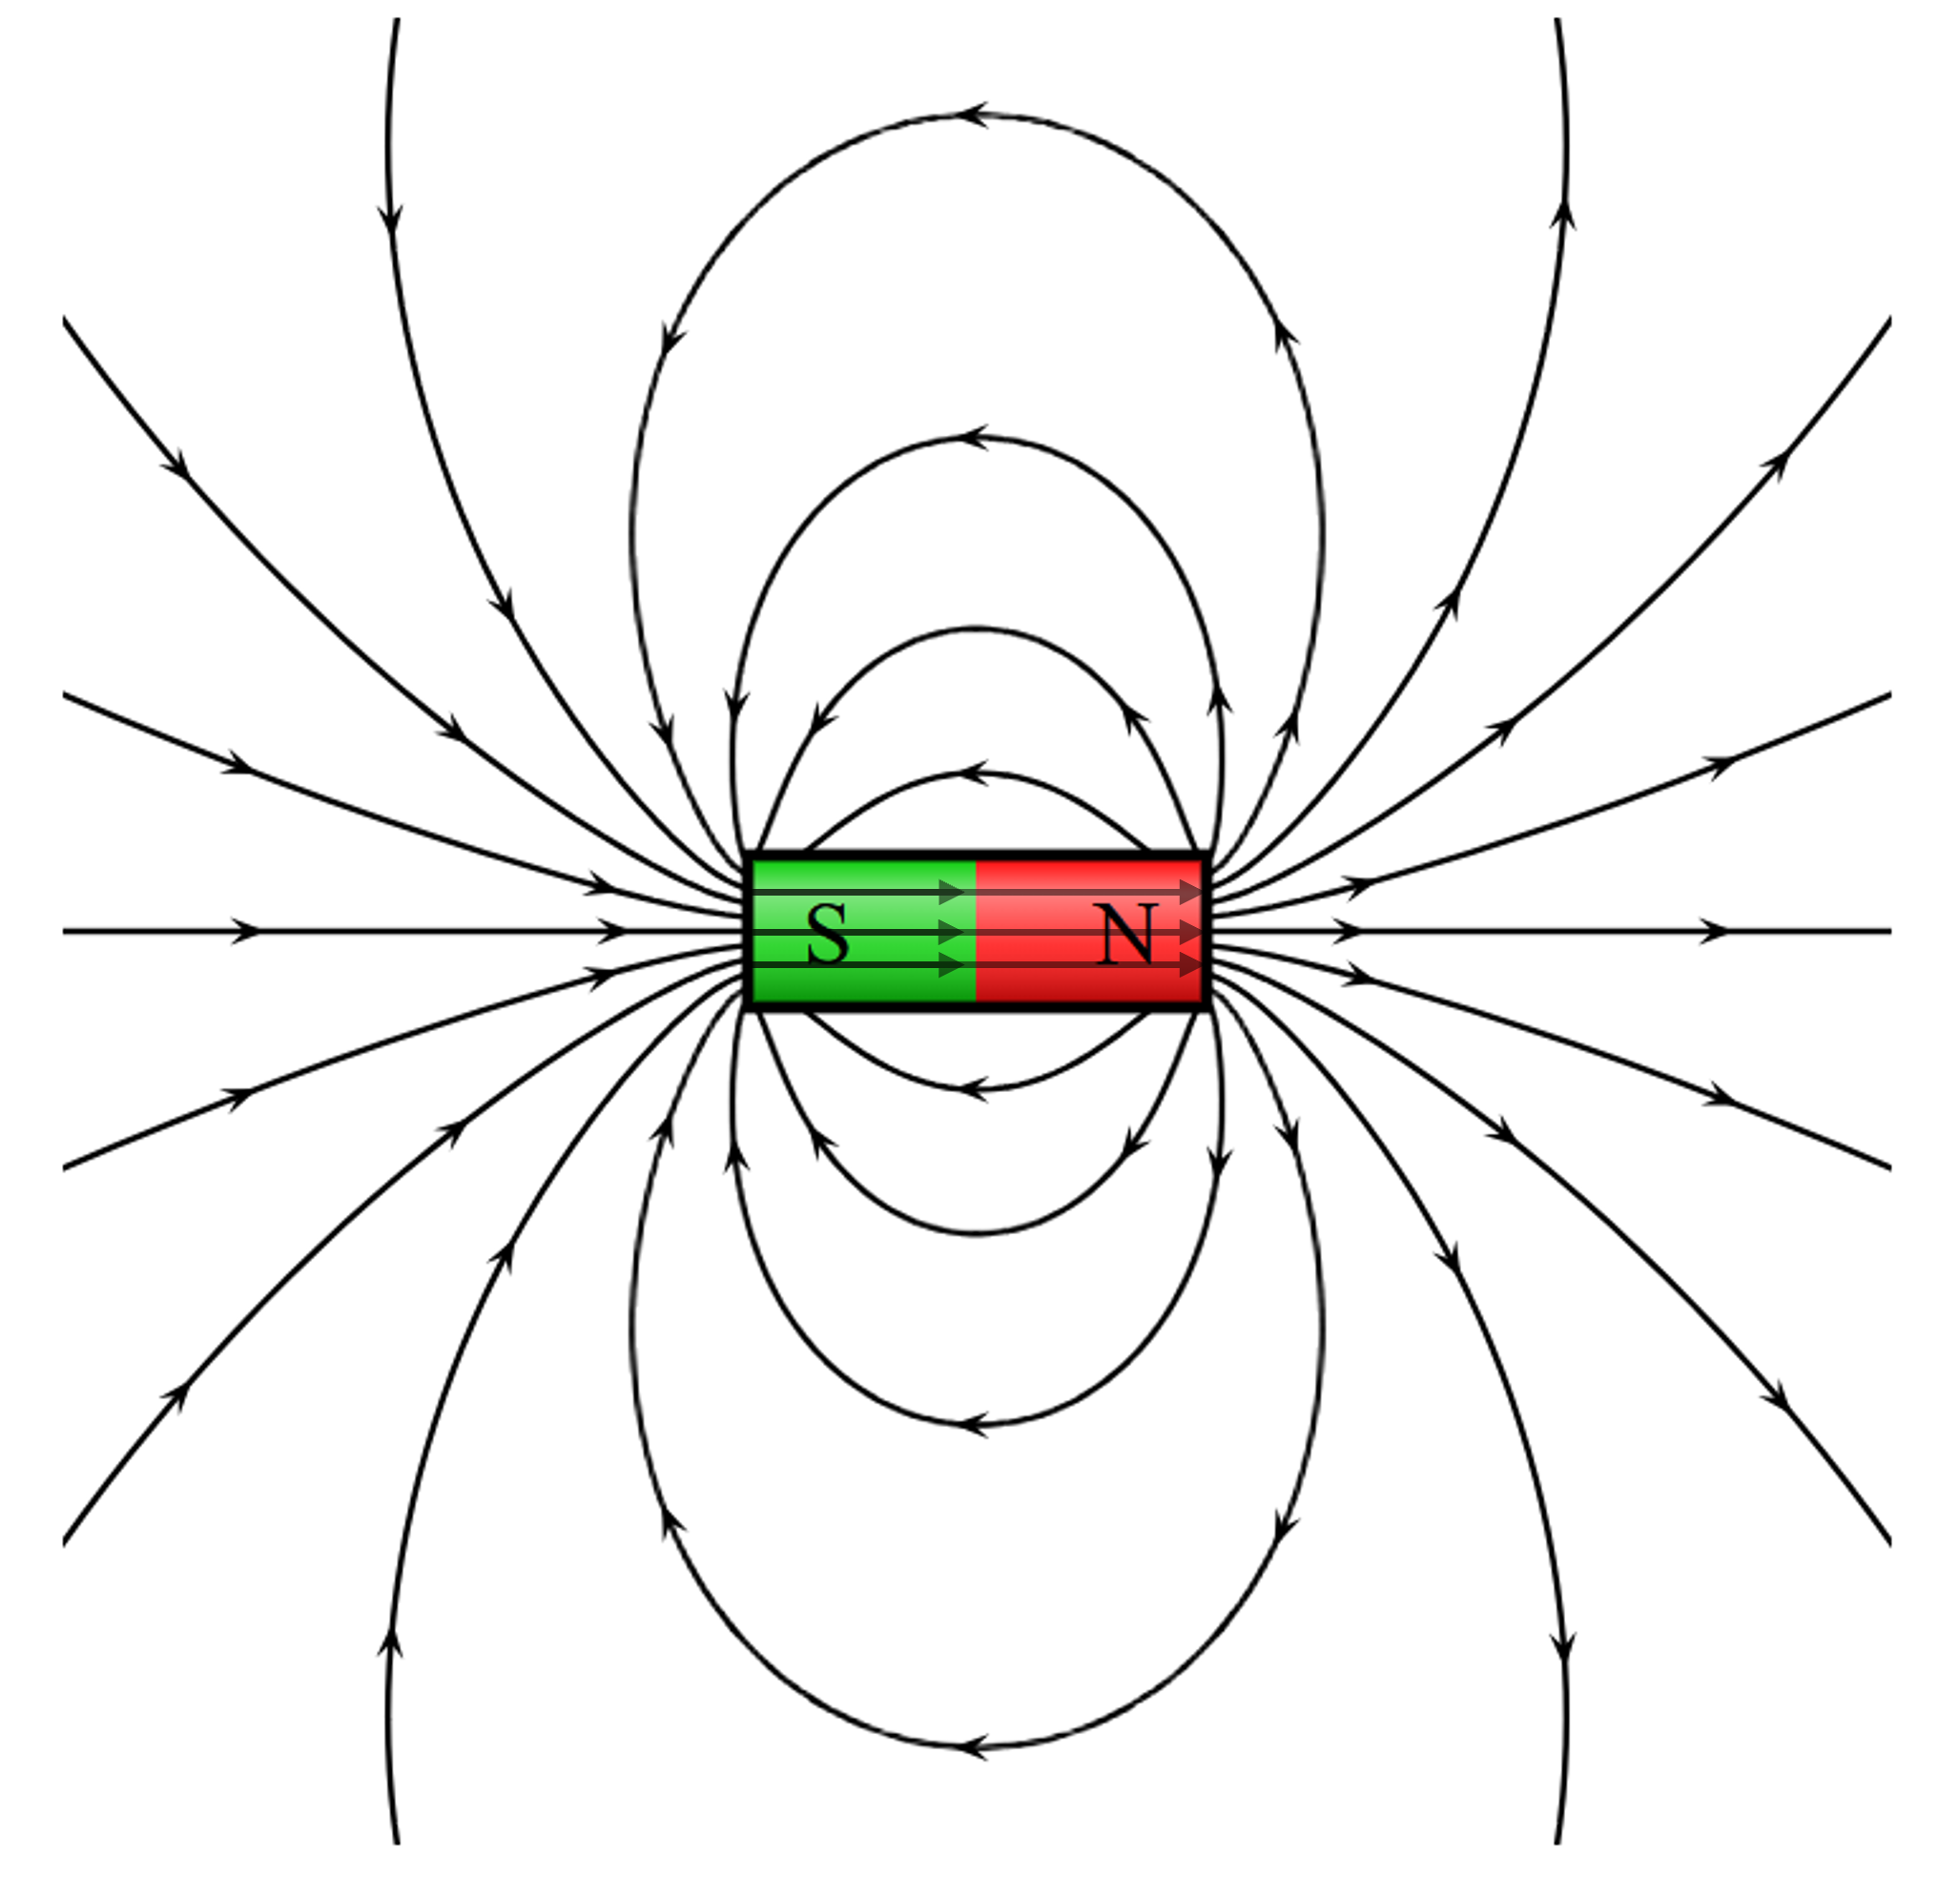
\includegraphics[height=6cm]{Bilder/magnetfeld_permanentmagnet.png}\\
  Stabmagnet
\end{minipage}
\end{center}
Beide Bilder zeigen auf den ersten Blick eine ähnliche Form. Was ist
trotzdem der wichtigste Unterschied zwischen den beiden Feldern?
\Antwortraum{3}
\begin{solution}
Die beiden Ladungen des elektrischen Dipols könnten auch für sich allein
existieren -- jede einzelne Ladung hätte dann ihr eigenes, einfaches
radiales Feld. Beim Stabmagneten ist das nicht möglich: Nord- und Südpol
lassen sich nicht voneinander trennen. Schneidet man den Magneten durch,
entstehen zwei neue, vollständige Magnete mit je einem Nord- und einem
Südpol -- nie ein isolierter einzelner Pol. Einen \glqq magnetischen
Monopol\grqq{}, das Gegenstück zu einer einzelnen elektrischen Ladung,
gibt es nicht.
\end{solution}
\end{taskbox}
\end{questions}

% =============================================================================
% Theorie: Regeln zum Zeichnen von Magnetfeldern (LZ1)
% =============================================================================
\begin{theoriebox}[Magnetfelder zeichnen]
\textbf{\emph{Regeln zum Zeichnen von Magnetfeldern:}}
\begin{itemize}[leftmargin=1.2cm,itemsep=0.2em]
  \item Feldlinien verlaufen \emph{ausserhalb} des Magneten vom Nordpol zum Südpol.
  \item Im \emph{Inneren} des Magneten schliessen sie sich vom Südpol zurück zum Nordpol -- jede Feldlinie ist eine geschlossene Kurve.
  \item Feldlinien kreuzen oder berühren sich nie.
  \item Die Richtung an einem Punkt entspricht der Richtung, in die der Nordpol einer dort platzierten Kompassnadel zeigt.
  \item Je dichter die Feldlinien gezeichnet sind, desto stärker ist das Feld an dieser Stelle.
\end{itemize}
\end{theoriebox}

\begin{questions}
\begin{taskbox}[Zeichenübung: Zwei Stabmagnete mit gleichnamigen Polen]
\question Zwei gleich starke Stabmagnete liegen sich gegenüber, dabei
zeigen \textbf{ihre Nordpole zueinander}. Zeichnen Sie -- unter Anwendung
der Regeln oben -- direkt in das Feld unten ein, wie die Feldlinien
zwischen und um die beiden Magnete verlaufen.
\begin{answerbox}
\vspace{4.5cm}
\begin{center}
\begin{tikzpicture}[>=Latex,scale=1]
  % linker Magnet: S (links) -- N (rechts, zeigt zur Mitte)
  \draw[thick] (-4.5,0) rectangle (-2,0.9);
  \draw[thick] (-3.25,0) -- (-3.25,0.9);
  \node at (-3.875,0.45) {S};
  \node at (-2.625,0.45) {N};
  % rechter Magnet: N (links, zeigt zur Mitte) -- S (rechts)
  \draw[thick] (2,0) rectangle (4.5,0.9);
  \draw[thick] (3.25,0) -- (3.25,0.9);
  \node at (2.625,0.45) {N};
  \node at (3.875,0.45) {S};
\end{tikzpicture}
\end{center}
\vspace{4.5cm}
\end{answerbox}
\begin{solution}
% Absichtlich FALSCHE Lösung zur Fehlersuche im Unterricht: Das Bild zeigt
% einfach die beiden unabhängigen Einzelfelder übereinandergelegt: Genau
% dadurch kreuzen sich die Feldlinien im Zwischenraum -- das ist der
% Fehler, den die Klasse finden soll (siehe Erläuterung unten).
\begin{center}
  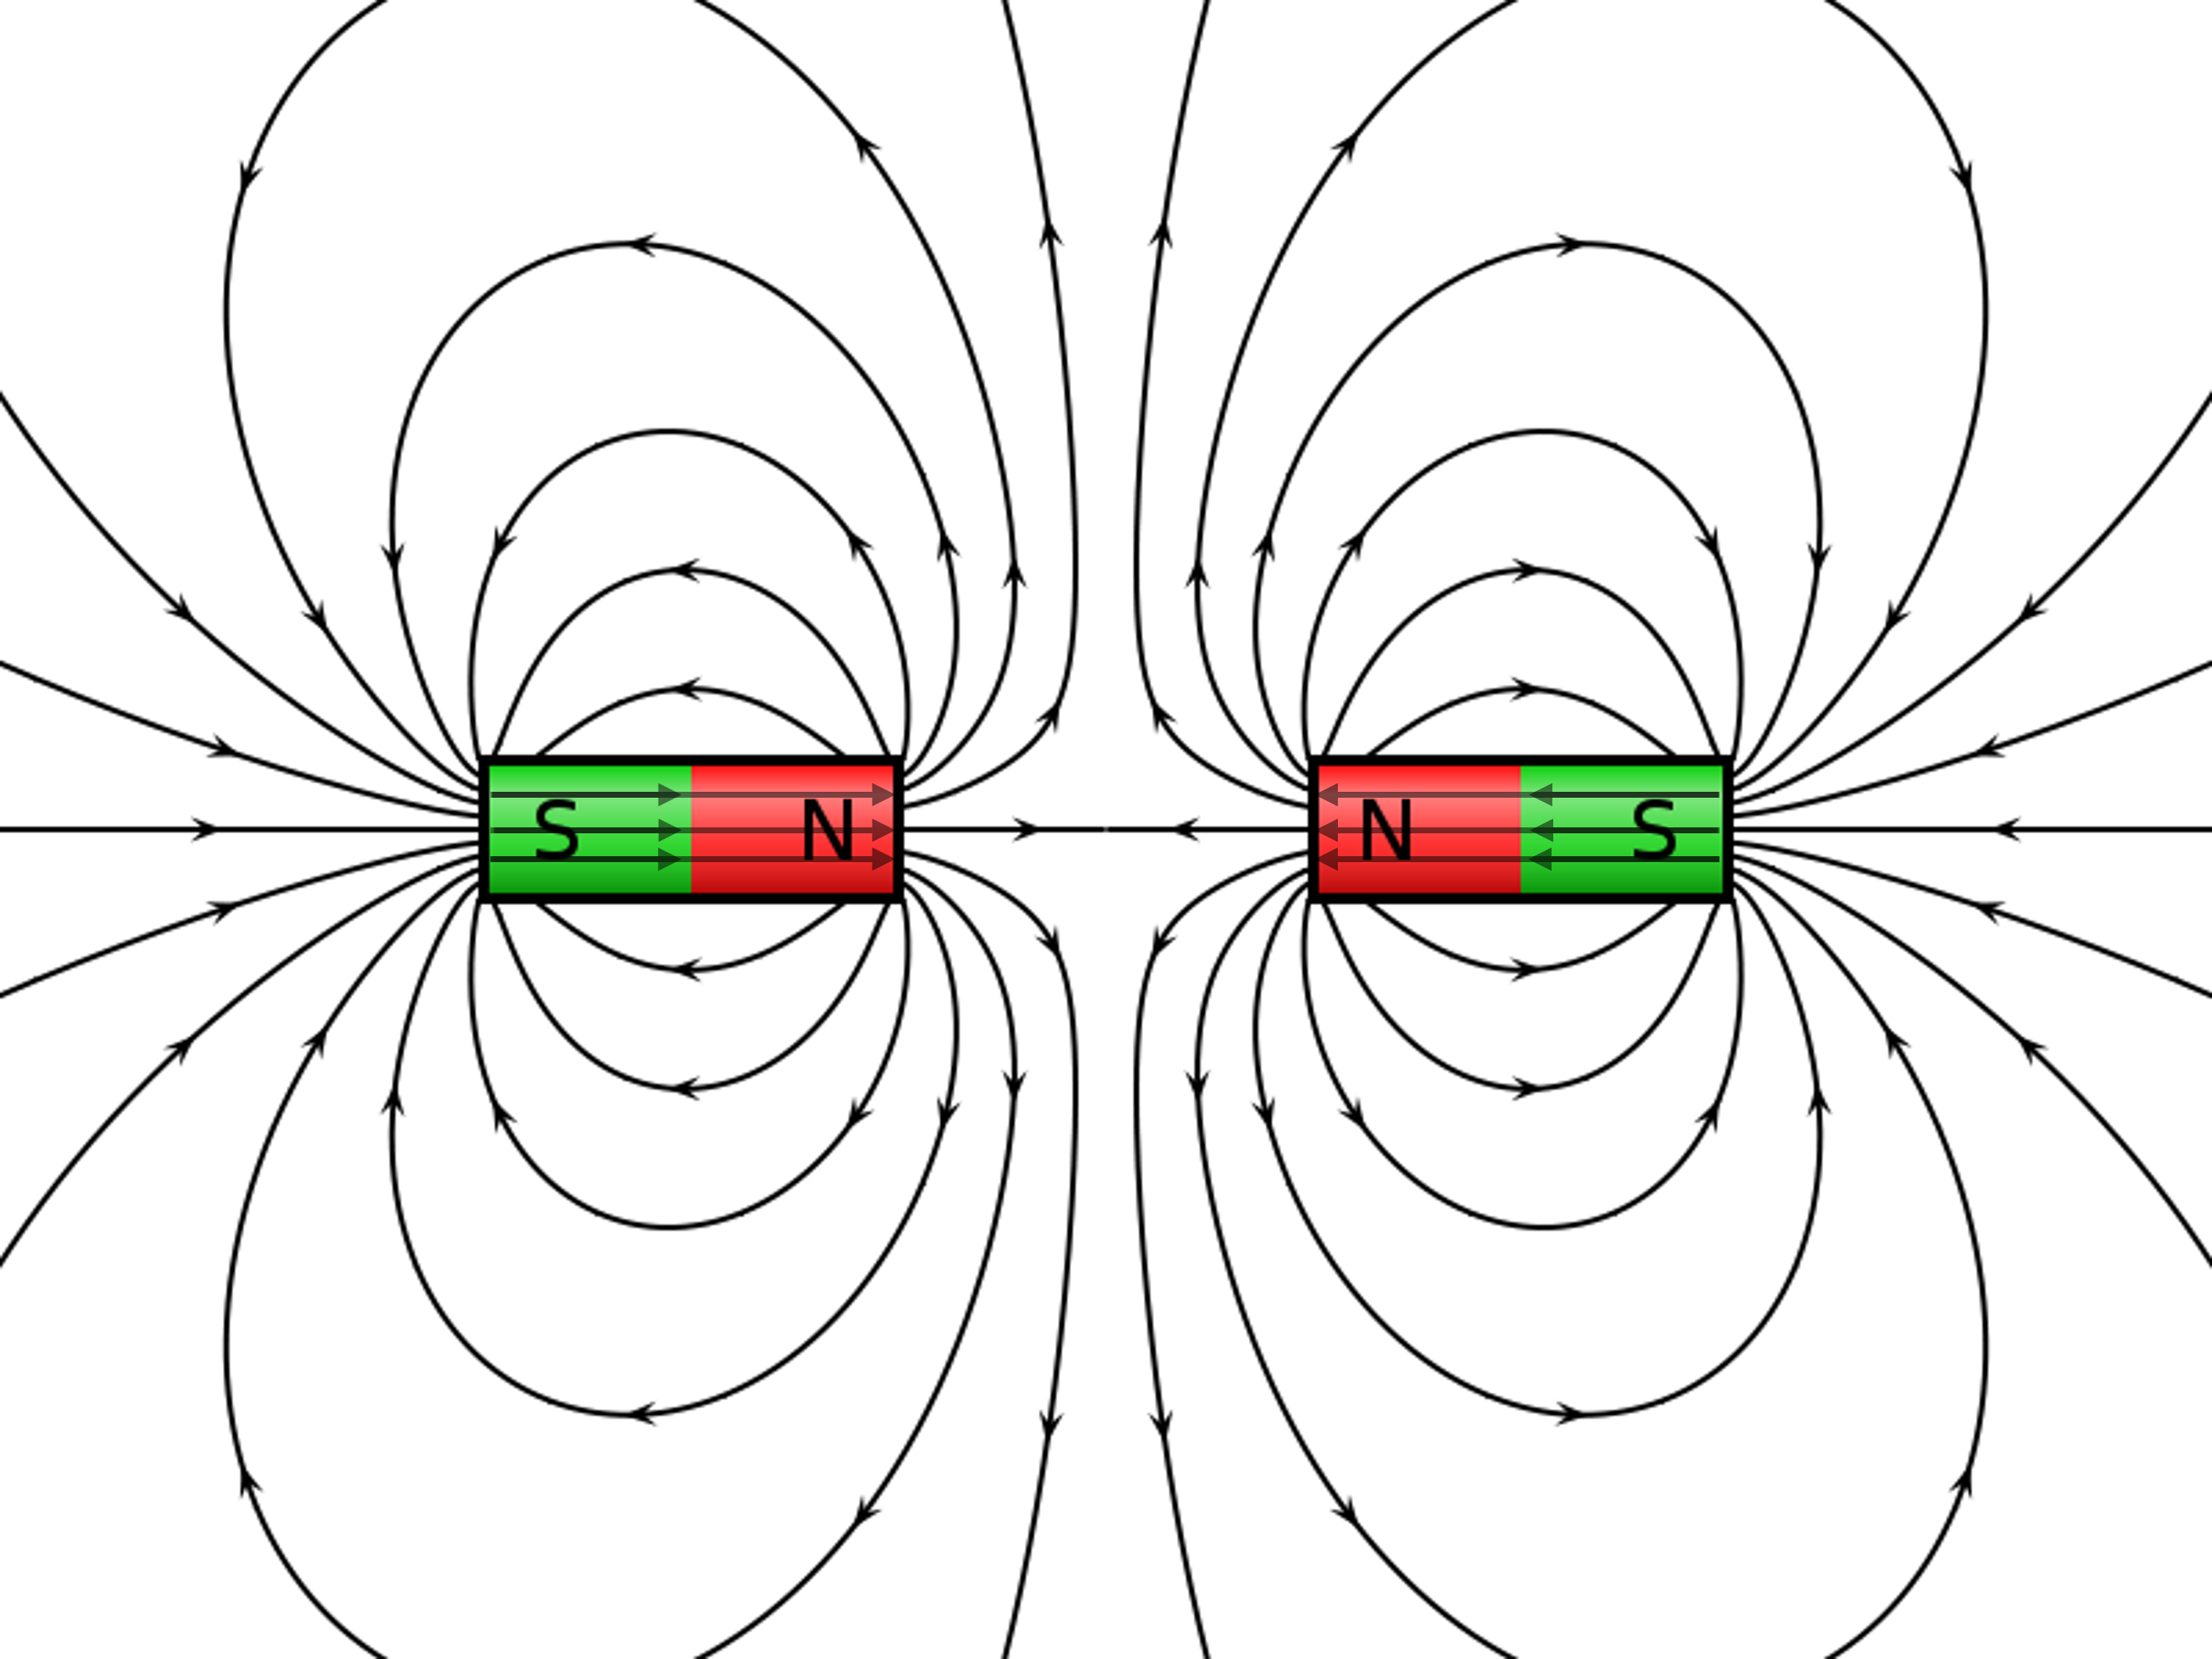
\includegraphics[width=8cm]{Bilder/Stabmagnet_gegenpolung.png}
\end{center}
\textbf{Fehlersuche:} Diese Lösung enthält absichtlich einen Fehler --
finden Sie ihn, bevor Sie weiterlesen.

Das Bild zeigt einfach die Feldlinien, die \emph{jeder Magnet für sich
allein} erzeugen würde, übereinandergelegt. Genau im Zwischenraum
\textbf{kreuzen sich} dadurch mehrere Feldlinien der beiden Magnete. Das
widerspricht der Regel, dass sich Feldlinien nie kreuzen dürfen --
ausserdem berücksichtigt das Bild gar nicht, dass sich die beiden
Magnete gegenseitig beeinflussen. Richtig ist stattdessen: Zwei
gleichnamige Pole stossen sich ab, die Feldlinien weichen im Zwischenraum
seitlich auseinander statt sich zu kreuzen, und in der Mitte entsteht ein
feldfreier Punkt (Nullstelle), an dem sich die Wirkungen beider Magnete
exakt aufheben.
\end{solution}
\end{taskbox}
\end{questions}

% =============================================================================
% Theorie: Das Erdmagnetfeld (LZ1)
% =============================================================================
\begin{theoriebox}[Das Erdmagnetfeld]
Auch die Erde selbst besitzt ein Magnetfeld, das in seiner Form demjenigen
eines riesigen Stabmagneten im Erdinneren ähnelt. Deshalb zeigt eine
Kompassnadel überall auf der Erde nach Norden.

\begin{center}
  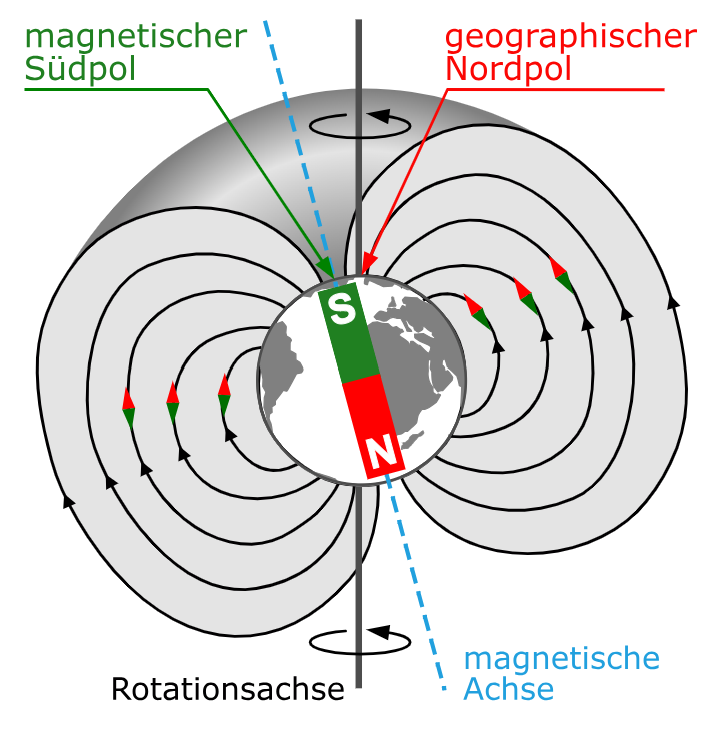
\includegraphics[width=6.5cm]{Bilder/erdmagnetfeld.png}
\end{center}
{\scriptsize Das Erdmagnetfeld: geografischer und magnetischer Nordpol
liegen nicht am selben Ort.}

\begin{hinweisbox}[Achtung, Verwechslungsgefahr]
Der \textbf{\emph{geografische Nordpol}} (die Drehachse der Erde) und der
\textbf{\emph{magnetische Nordpol}} sind \emph{nicht} derselbe Ort. Da sich
Feldlinien vom magnetischen Nordpol weg und zum magnetischen Südpol hin
bewegen, eine Kompassnadel aber am geografischen Nordpol nach Norden zeigt,
liegt dort tatsächlich der \textbf{magnetische Südpol} des Erdmagnetfelds.
\end{hinweisbox}
\end{theoriebox}

% =============================================================================
% Überleitung: Die Geschichte von Ørsted
% =============================================================================
\begin{beispielbox}[Die Geschichte von Ørsted]
\begin{center}
  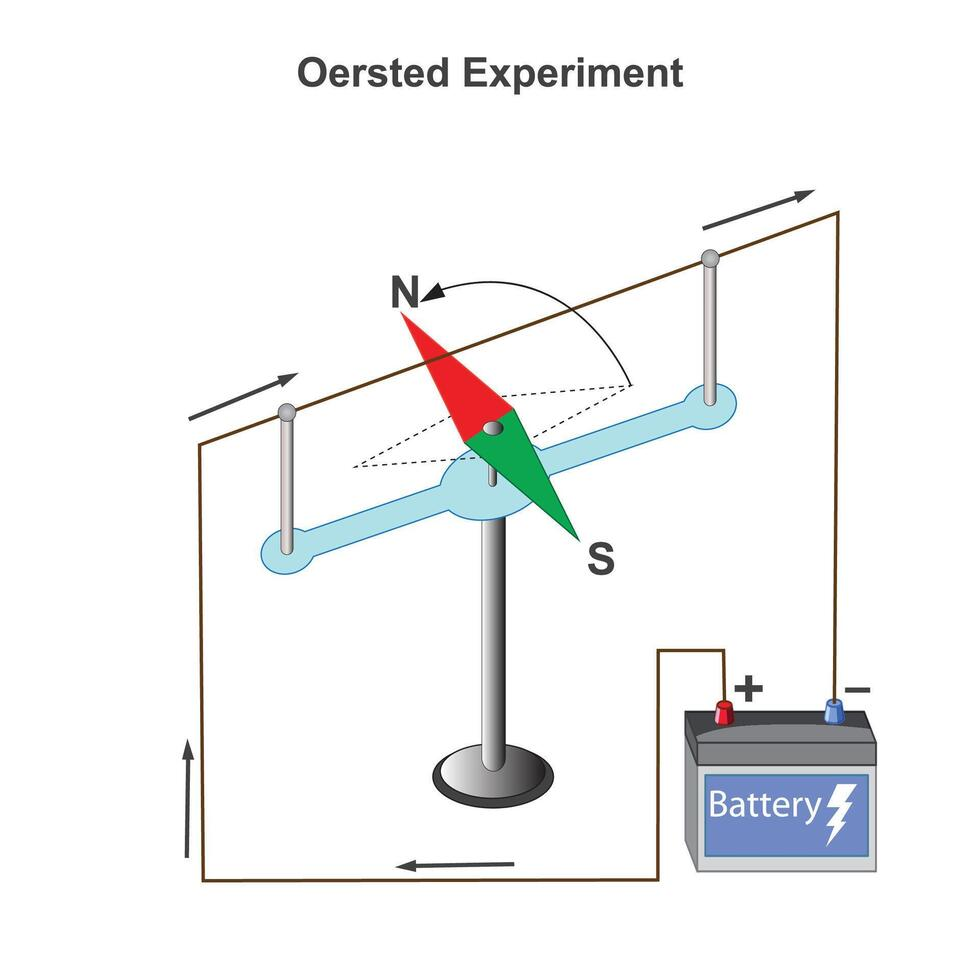
\includegraphics[width=7cm]{Bilder/oersted-experiment-showed-electric-current-creates-a-magnetic-field-fundamental-in-electromagnetism-s-development-p.jpg}
\end{center}
Im Jahr 1820 hielt der dänische Physiker Hans Christian Ørsted eine
Vorlesung, bei der zufällig eine Kompassnadel in der Nähe eines
stromdurchflossenen Drahtes lag. Als er den Stromkreis schloss, schlug die
Kompassnadel aus, obwohl niemand einen Magneten in die Nähe gebracht
hatte. Bis zu diesem Moment galten Elektrizität und Magnetismus als zwei
völlig getrennte Phänomene -- Ørsteds Zufallsbeobachtung war der erste
direkte Beweis dafür, dass fliessender Strom selbst ein Magnetfeld
erzeugt.

Genau diesen Effekt untersuchen Sie jetzt selbst.
\end{beispielbox}

\begin{hinweisbox}[Achtung, wichtiger Unterschied]
Ab jetzt betrachten wir keine \textbf{Permanentmagnete} (Stabmagnete)
mehr, sondern \textbf{Elektromagnete}: Magnetfelder, die durch
elektrischen Strom erzeugt werden. Ein Elektromagnet besitzt
\textbf{keine festen Pole} -- die Richtung seines Feldes hängt direkt
von der Stromrichtung ab und lässt sich jederzeit durch Umpolen
umkehren.
\end{hinweisbox}

% =============================================================================
% Baukasten-Experiment (Partnerarbeit): Feld bei Leiter und Spule
% =============================================================================
\begin{questions}
\begin{groupbox}[Baukasten-Experiment (Partnerarbeit): Feld bei Leiter und Spule]
% TODO: Foto des Baukastens/Versuchsaufbaus einfügen, sobald vorhanden
% (noch nicht erstellt -- keine eigene Skizze an dieser Stelle).
\question Sie erhalten einen Baukasten mit einem Stromkreis, der einen
geraden Stableiter und eine Spule enthält, sowie mehrere kleine
Kompassnadeln. Der Stromkreis wird über einen Schalter eingeschaltet,
dessen \glqq On\grqq-Taste Sie \textbf{gedrückt halten} müssen, damit
Strom fliesst. Lassen Sie los, fliesst kein Strom mehr. Mit demselben
Schalter können Sie ausserdem die Stromrichtung umpolen.
\begin{parts}
  \part[4] Untersuchen Sie mit den Kompassnadeln \textbf{beide} Bauteile
  nacheinander. Beschreiben Sie für \textbf{jedes} der beiden Felder, wie
  sich die Nadeln ausrichten: beim geraden Stableiter in verschiedenen
  Abständen rund um den Draht (wie bei Ørsted); bei der Spule innerhalb
  der Spule.
  \Antwortraum{4}
  \begin{solution}
  \textbf{Gerader Leiter:} Die Kompassnadeln stellen sich tangential zu
  gedachten Kreisen um den Draht -- je näher am Draht, desto stärker der
  Ausschlag.

  \textbf{Spule:} Im Inneren zeigen alle Kompassnadeln in dieselbe
  Richtung entlang der Spulenachse (ein starkes, einheitliches Feld).
  \end{solution}

  \part[3] Kehren Sie jetzt die Stromrichtung im Stromkreis um. Was
  verändert sich \textbf{sowohl} am Feld des geraden Leiters \textbf{als
  auch} am Feld der Spule?
  \Antwortraum{3}
  \begin{solution}
  \textbf{Gerader Leiter:} Die Feldrichtung kehrt sich vollständig um --
  alle Kompassnadeln um den Draht schlagen in die jeweils entgegengesetzte
  Richtung aus.

  \textbf{Spule:} Ebenfalls vollständige Umkehr -- die Kompassnadeln im
  Inneren zeigen jetzt in die Gegenrichtung, das Feld der Spule zeigt
  also insgesamt in die entgegengesetzte Richtung.
  \end{solution}
\end{parts}
\end{groupbox}
\end{questions}

% =============================================================================
% Theorie: Rechte-Faust-Regel und Formeln (LZ2, LZ3)
% =============================================================================
\begin{theoriebox}[Das Magnetfeld des geraden Leiters]
Von oben betrachtet (Blick entlang des Drahtes) bilden die Feldlinien um
einen stromdurchflossenen, geraden Leiter \textbf{\emph{konzentrische
Kreise}}.

Die Richtung des Feldes bestimmen Sie mit der
\textbf{\emph{Rechte-Faust-Regel}}: Zeigt der Daumen der rechten Hand in
Stromrichtung, geben die gekrümmten Finger die Richtung des Magnetfelds an.

\begin{center}
  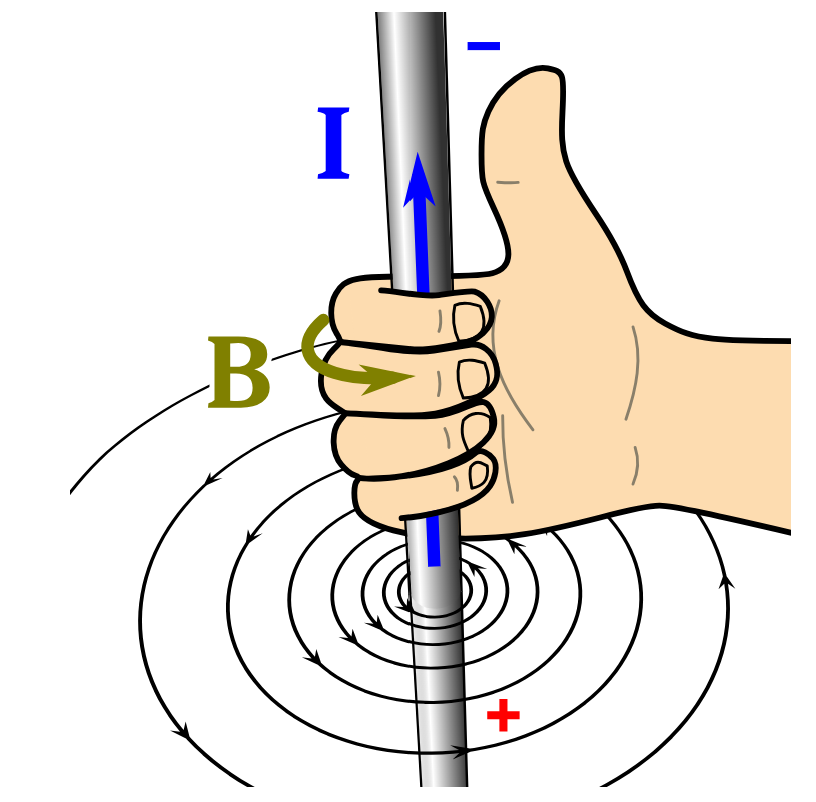
\includegraphics[width=6cm]{Bilder/leiter.png}
\end{center}
{\scriptsize Rechte-Faust-Regel für den geraden Leiter: Daumen zeigt in
Stromrichtung $I$, die gekrümmten Finger zeigen die Richtung von $\vec B$.}

\begin{formelbox}[Magnetische Flussdichte: gerader Leiter]
\[
  B = \frac{\mu_0}{2\pi}\cdot\frac{I}{r}
\]
$\mu_0 = 4\pi\cdot10^{-7}\,\si{\newton\per\ampere\squared}$ (magnetische
Feldkonstante); Einheit von $B$: $\si{\tesla}$ (Tesla, benannt nach
Nikola Tesla). Herleitung der Einheit (im Plenum):
\vspace{1.3cm}
\end{formelbox}
\end{theoriebox}

\begin{theoriebox}[Das Magnetfeld der Spule]
Reiht man viele stromdurchflossene Windungen dicht aneinander, addieren
sich ihre Felder zu einem starken, im Inneren nahezu homogenen Magnetfeld
entlang der ganzen Spulenachse -- genau das haben Sie im
Baukasten-Experiment beobachtet.

\begin{center}
  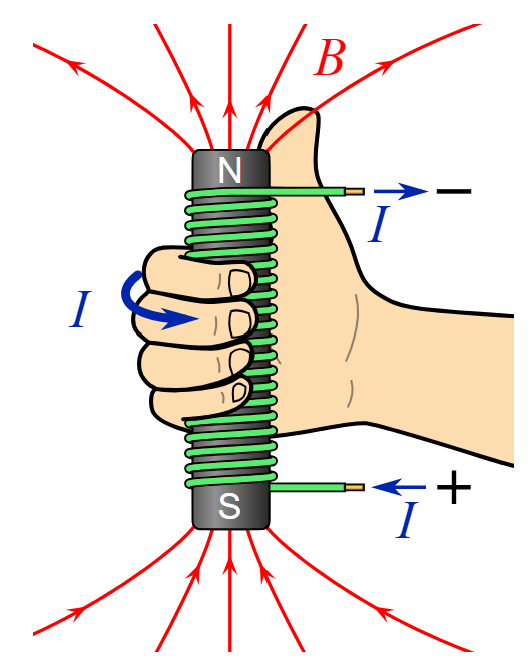
\includegraphics[width=7.5cm]{Bilder/spule.png}
\end{center}
{\scriptsize Rechte-Faust-Regel für die Spule: Zeigen die gekrümmten Finger
in Stromrichtung (Windungsrichtung), zeigt der Daumen in Richtung des
Feldes im Innern der Spule.}

\begin{formelbox}[Magnetische Flussdichte: Spule]
\[
  B = \mu_0\cdot\frac{N}{l}\cdot I = \mu_0\cdot n\cdot I
\]
$N$: Windungszahl, $l$: Spulenlänge, $n=\frac{N}{l}$: Windungsdichte;
Einheit von $B$: $\si{\tesla}$.
\end{formelbox}

\begin{center}
  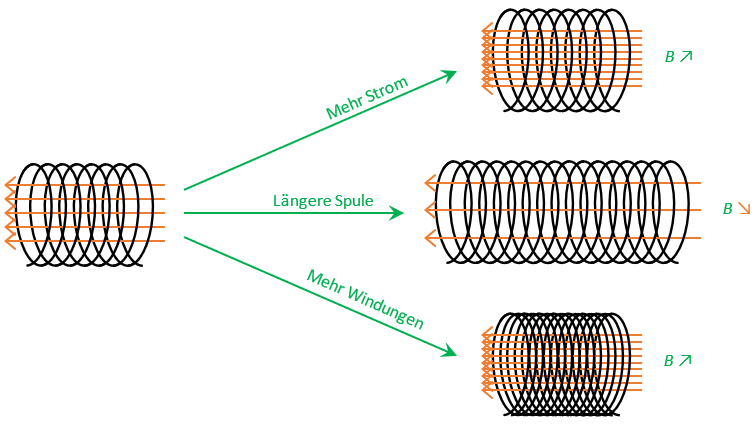
\includegraphics[width=9cm]{Bilder/Einflussgroessen_spuhle.png}
\end{center}
{\scriptsize Einflussgrössen auf $B$: mehr Strom oder mehr Windungen
vergrössern $B$, eine längere Spule (bei gleicher Windungszahl)
verkleinert $B$.}

Das homogene Feld im Inneren einer Spule ist die magnetische Entsprechung
des homogenen elektrischen Feldes im Inneren eines Plattenkondensators.

Auch das eingangs gezeigte Erdmagnetfeld entsteht nach genau diesem
Prinzip: Schraubenförmige Strömungen im flüssigen äusseren Erdkern wirken
wie unzählige kleine Spulen und erzeugen dadurch das Magnetfeld der Erde.

\begin{center}
  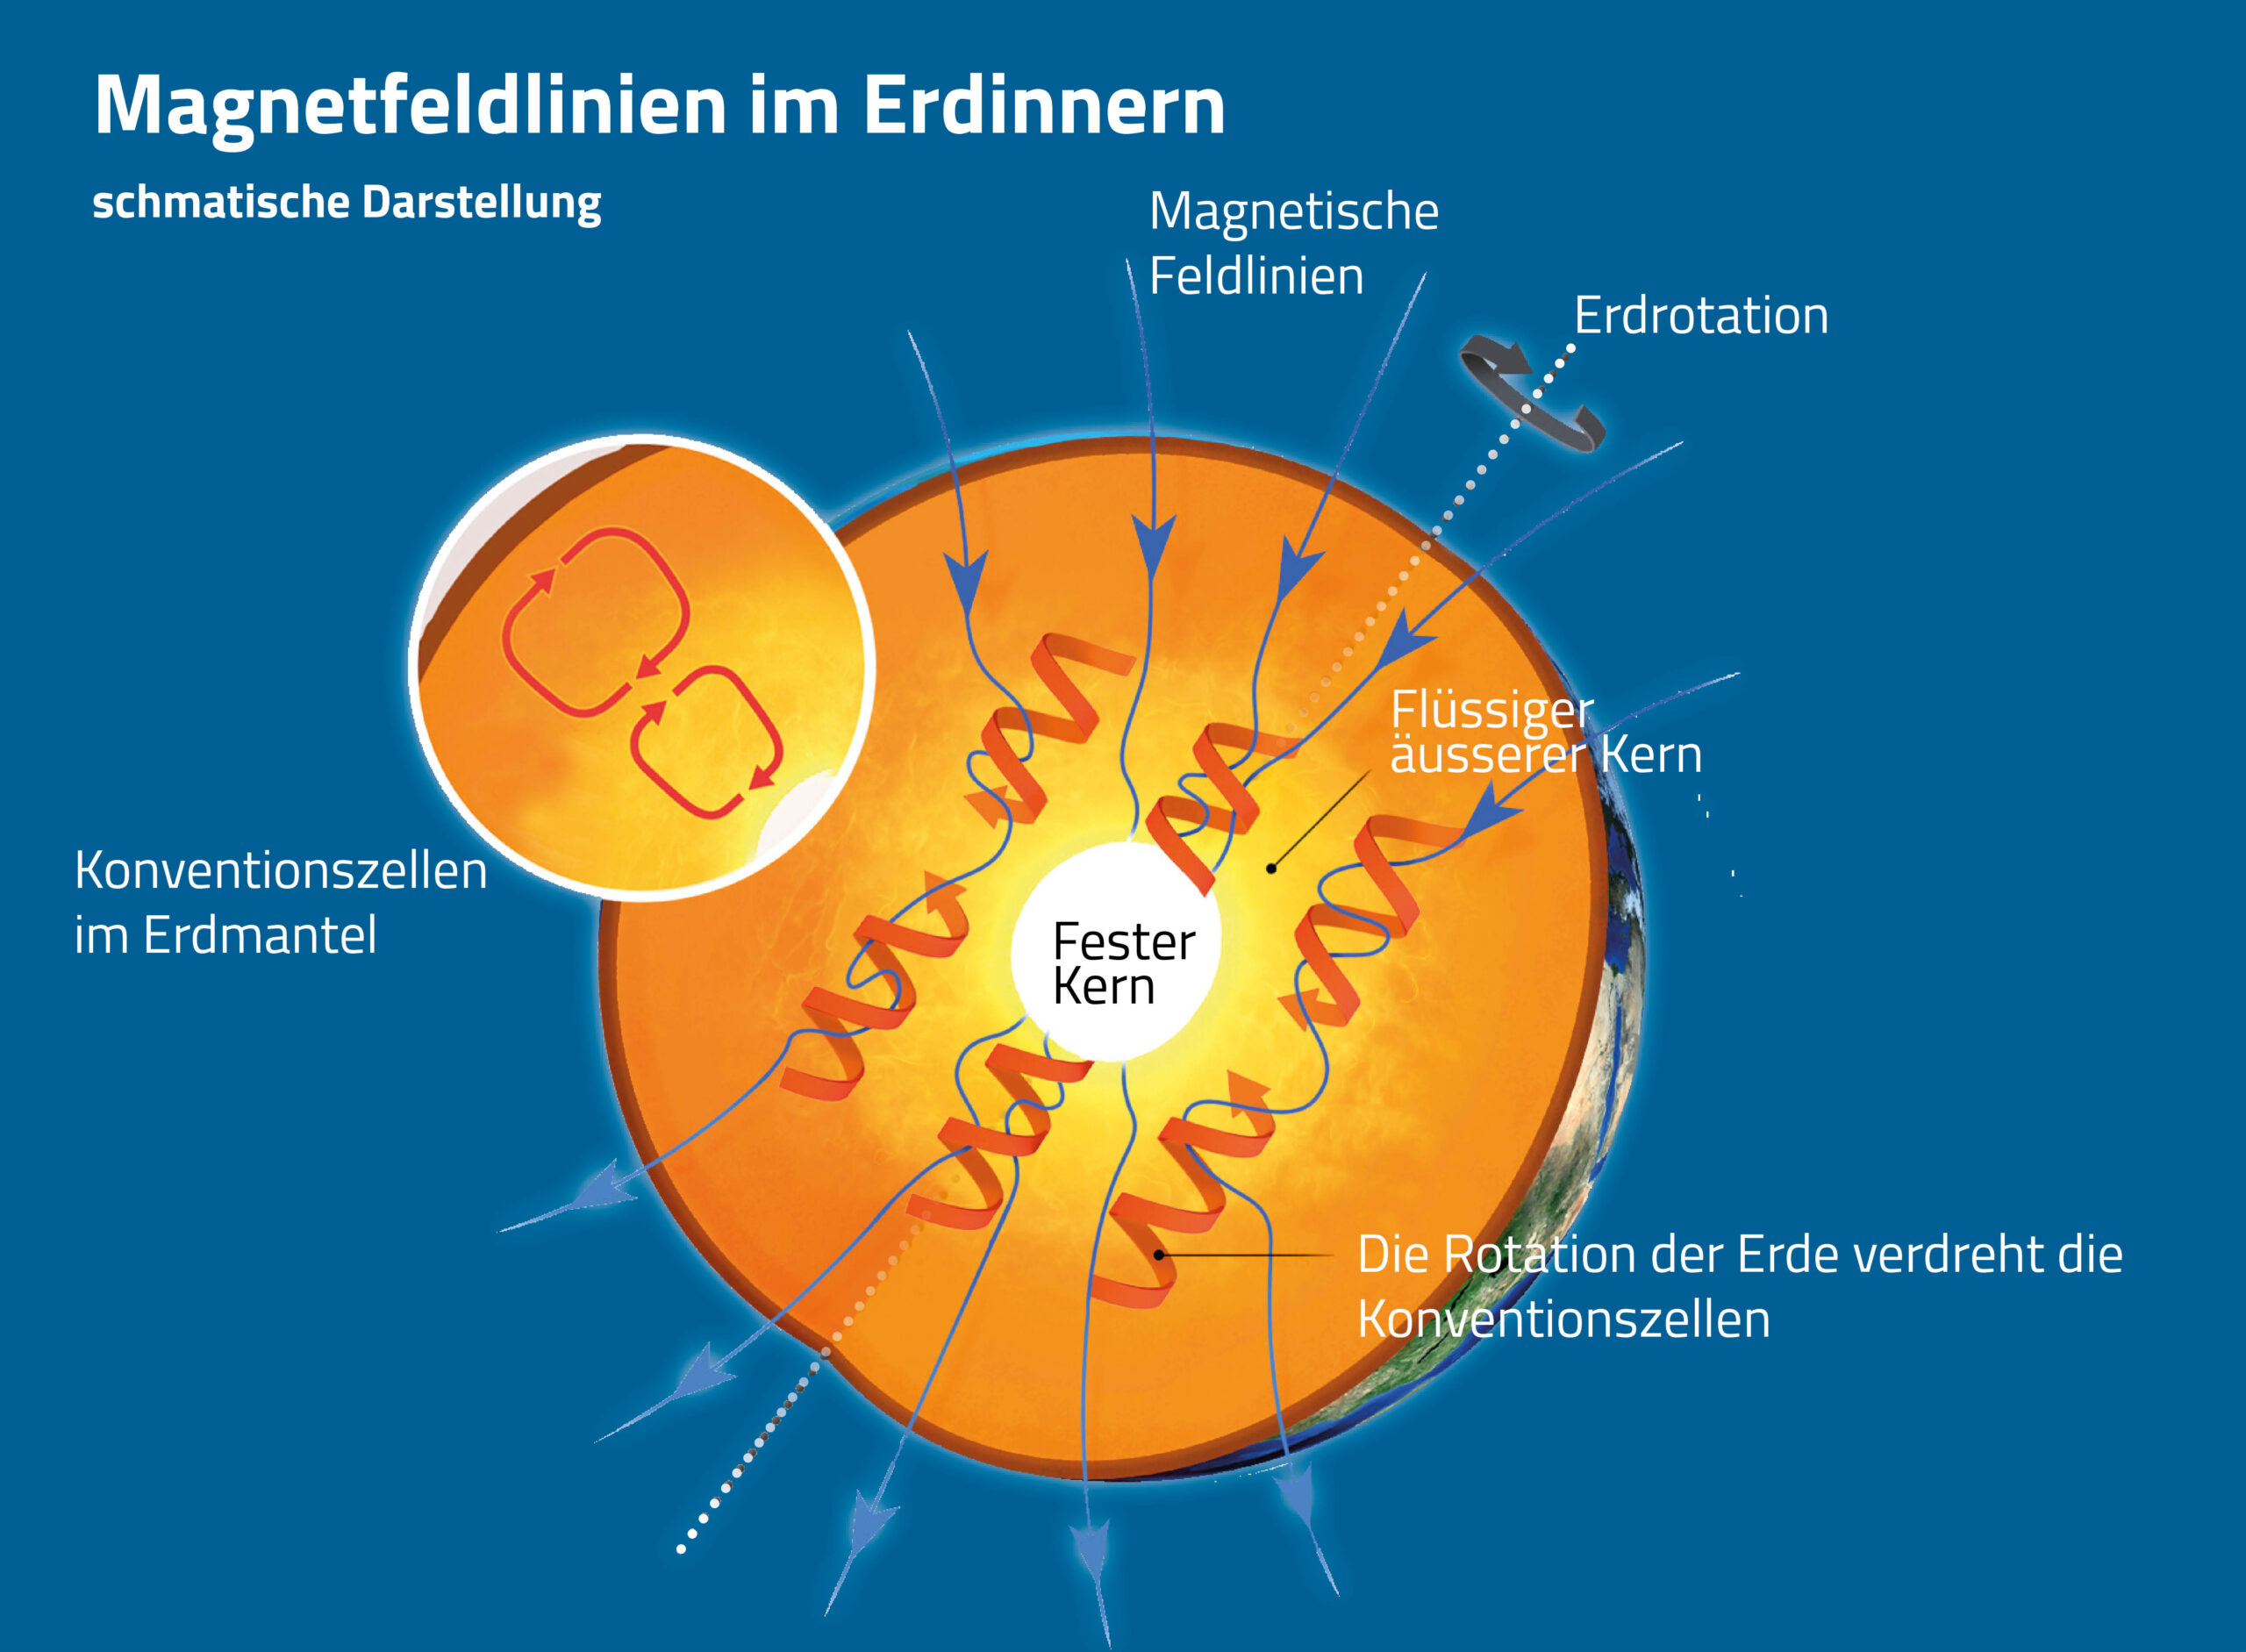
\includegraphics[width=7.5cm]{Bilder/Erdmagnetfeld-innen-scaled.jpg}
\end{center}
{\scriptsize Ursache des Erdmagnetfelds: schraubenförmige Strömungen im
flüssigen äusseren Kern wirken wie viele kleine Spulen.}
\end{theoriebox}

\begin{hinweisbox}[Achtung, Verwechslungsgefahr]
Es gibt \textbf{zwei verschiedene} Rechte-Faust-Regeln: Beim
\textbf{geraden Leiter} zeigt der \textbf{Daumen} in Stromrichtung, die
\textbf{Finger} zeigen die Feldrichtung. Bei der \textbf{Spule} ist es
umgekehrt: Die \textbf{Finger} zeigen in Stromrichtung (Windungsrichtung),
der \textbf{Daumen} zeigt in Richtung des Feldes im Innern. Prüfen Sie bei
jeder Aufgabe zuerst, um welchen Fall es sich handelt.
\end{hinweisbox}

\begin{questions}
\begin{taskbox}[Frage: Leiter- und Spulenfeld im Vergleich]
\question Wie unterscheidet sich das Magnetfeld eines geraden,
stromdurchflossenen Leiters von demjenigen im Innern einer
stromdurchflossenen Spule?
\Antwortraum{2}
\begin{solution}
Beim geraden Leiter bilden die Feldlinien konzentrische Kreise um den
Draht; die Feldstärke nimmt mit wachsendem Abstand $r$ vom Draht ab. Im
Innern einer Spule dagegen verlaufen die Feldlinien parallel zur
Spulenachse, und das Feld ist nahezu \textbf{\emph{homogen}}: Die
Feldstärke ist im ganzen Innenraum (fernab der Enden) praktisch überall
gleich gross.
\end{solution}
\end{taskbox}
\end{questions}

\begin{questions}
\begin{taskbox}[Frage: Richtung des Spulenfelds]
\question Betrachten Sie die beiden Spulen unten, seitlich aufgeschnitten
gezeichnet. Beide sind an derselben Batterie-Polung angeschlossen ($+$
jeweils links, $-$ jeweils rechts), aber \textbf{unterschiedlich
gewickelt}: Spule A ist rechtsgewickelt, Spule B linksgewickelt.
\begin{center}
\begin{minipage}[t]{7cm}\centering
  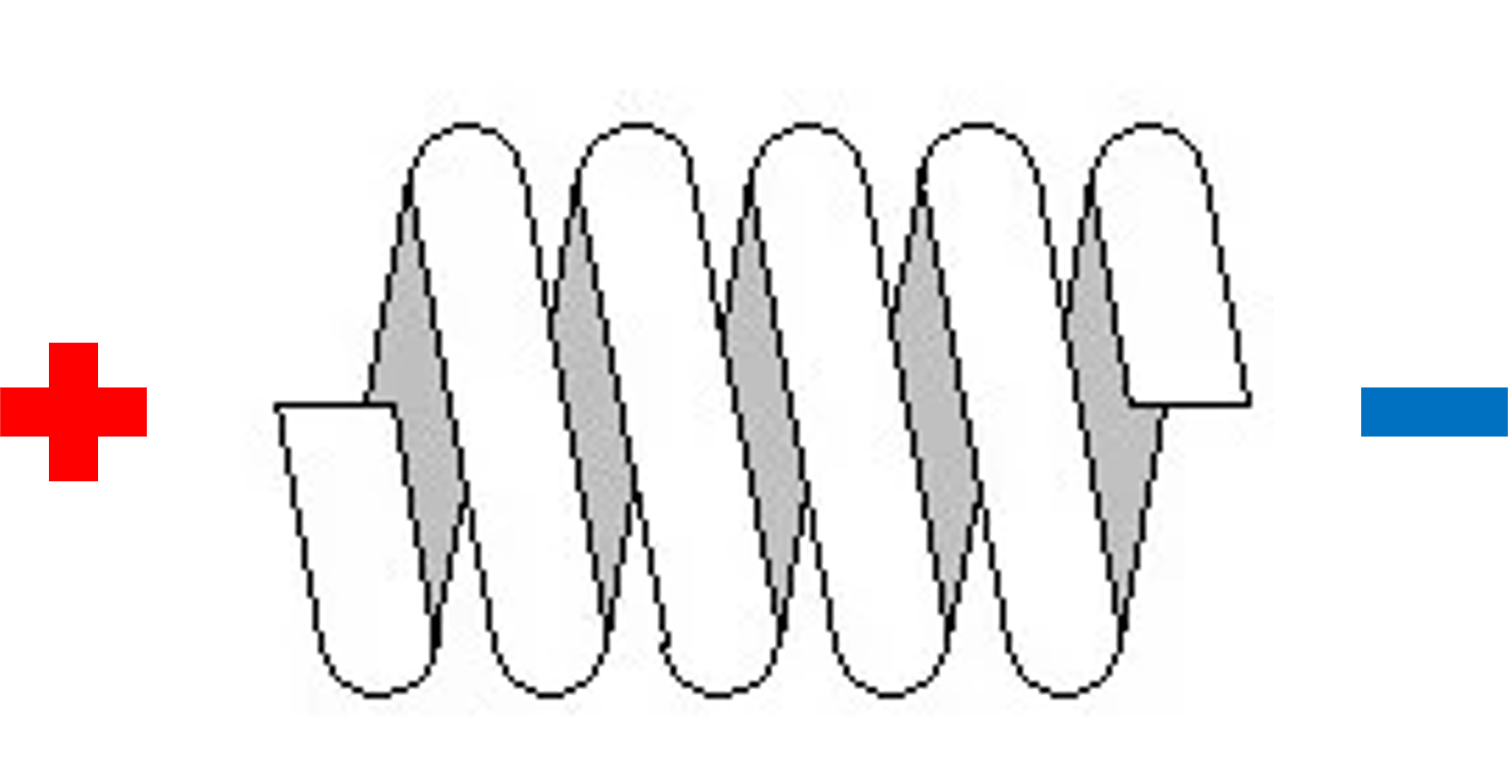
\includegraphics[width=6.5cm]{Bilder/windung_rechts.png}\\
  Spule A (rechtsgewickelt)
\end{minipage}\hfill
\begin{minipage}[t]{7cm}\centering
  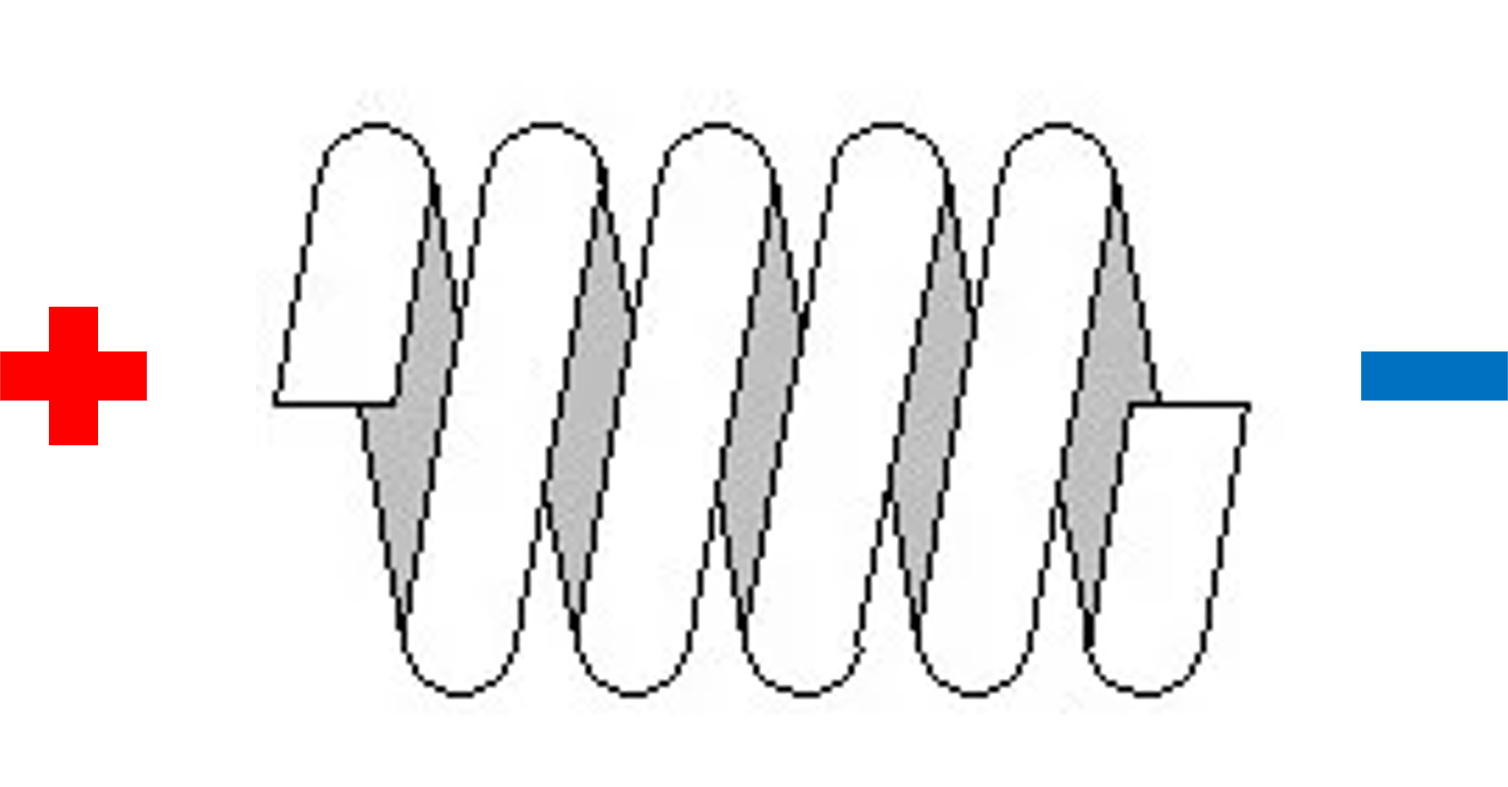
\includegraphics[width=6.5cm]{Bilder/windung_links.png}\\
  Spule B (linksgewickelt)
\end{minipage}
\end{center}

Welche \textbf{zwei} Faktoren legen zusammen fest, in welche Richtung
entlang der Spulenachse das Magnetfeld im Innern einer Spule zeigt? Fahren
Sie ausserdem mit den gekrümmten Fingern der rechten Hand dem
gezeichneten Draht in Stromrichtung (von $+$ nach $-$) entlang: Wohin
zeigt der Daumen bei Spule A, wohin bei Spule B?
\Antwortraum{3}
\begin{solution}
Erstens die \textbf{\emph{Stromrichtung}} (Polung, d.\,h. welche Klemme
der Batterie an welches Spulenende angeschlossen ist) und zweitens die
\textbf{\emph{Windungsrichtung}} der Spule (im oder gegen den
Uhrzeigersinn gewickelt). Kehrt man nur einen der beiden Faktoren um,
kehrt sich die Feldrichtung im Innern der Spule um; kehrt man beide
gleichzeitig um, zeigt das Feld wieder in dieselbe Richtung wie zuvor.

Bei Spule A und Spule B ist die Stromrichtung (Polung) identisch, nur die
Windungsrichtung ist entgegengesetzt -- nach obiger Regel zeigt das Feld
im Innern der beiden Spulen deshalb in \textbf{entgegengesetzte}
Richtungen: Finden Sie mit der rechten Hand am Bild heraus, wohin der
Daumen bei Spule A zeigt -- bei Spule B zeigt er dann in die genau
entgegengesetzte Richtung.
\end{solution}
\end{taskbox}
\end{questions}

\end{document}
